%
% drei.tex
%
% (c) 2018 Prof Dr Andreas Müller, Hochschule Rapperswil
%
\documentclass[tikz]{standalone}
\usepackage{times}
\usepackage{amsmath}
\usepackage{txfonts}
\usepackage[utf8]{inputenc}
\usepackage{graphics}
\usetikzlibrary{arrows,intersections}
\usetikzlibrary{math}
\begin{document}
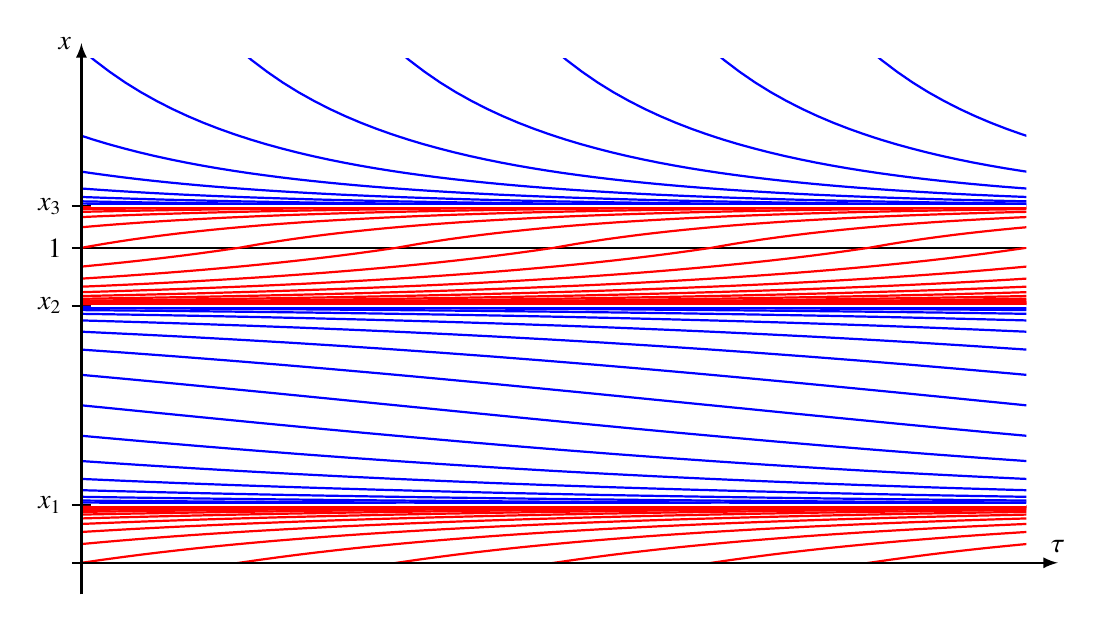
\begin{tikzpicture}[thick, >= latex, scale=4]

\tikzmath{
	real \a, \b, \xone, \xtwo, \xthree;
	\a = sqrt(0.25 - 0.15);
	\b = sqrt(0.25 + 0.15);
	\xone = 0.5 - \a;
	\xtwo = 0.5 + \a;
	\xthree = 0.5 + \b;
	real \taua, \taub, \z;
	\taua = 0.5 * ln((1+2*\a)/(1-2*\a)) / \a;
	\z = \b / (2 * \xthree - 1.5);
	\taub = 0.5 * ln((1+\z)/(1-\z)) / \b;
}

\draw (-0.03,{\xone})--(0.03,{\xone});
\draw (-0.03,{\xtwo})--(0.03,{\xtwo});
\draw (-0.03,{\xthree})--(0.03,{\xthree});

\node at (-0.03,{\xone}) [left] {$x_1$};
\node at (-0.03,{\xtwo}) [left] {$x_2$};
\node at (-0.03,{\xthree}) [left] {$x_3$};

\draw[line width=0.5] (0,1)--(3,1);
\draw (-0.03,1)--(0.03,1);
\node at (-0.03,1) [left] {$1$};

% oberhalb von x_3
\begin{scope}
\clip (0,0) rectangle (3,1.6);
\foreach\translate in {-8,-7,...,5}{
	\draw[color=blue,domain=0.1:5,samples=100]
		plot ({\x+\translate/2},{0.5+\b/tanh(\b*\x)});
}
\end{scope}

% zwischen 1 und x_3
\begin{scope}
\clip (0,1) rectangle (3,{\xthree});
\foreach\translate in {-8,-7,...,5}{
	\draw[color=red,domain=0.1:5,samples=100]
		plot ({\x+\translate/2-\taub},{2*\xthree-(0.5+\b/tanh(\b*\x))});
}
\end{scope}

% zwischen x_2 und 1
\begin{scope}
\clip (0,0) rectangle (3,1.0);
\foreach\translate in {0,1,...,20}{
	\draw[color=red,domain=-8:-2,samples=100]
		plot ({\x+\translate/2+\taua},{0.5-\a / tanh(\a*\x)});
}
\end{scope}

% zwischen x_1 und x_2
\begin{scope}
\clip (0,0) rectangle (3,1.6);
\foreach \translate in {-8,-7,...,10}{
	\draw[color=blue,domain=-8:8,samples=100]
		plot ({\x+\translate},{0.5-\a * tanh(\a*\x)});
}
\end{scope}

% zwischen 0 und x_1
\begin{scope}
\clip (0,0) rectangle (3,1.0);
\foreach\translate in {-14,-13,...,1}{
	\draw[color=red,domain=2:8,samples=100]
		plot ({\x+\translate/2-0.3574},{0.5-\a / tanh(\a*\x)});
}
\end{scope}

\draw[color=white] (0.03,{\xone})--(3.0,{\xone});
\draw[color=white] (0.03,{\xtwo})--(3.0,{\xtwo});
\draw[color=white] (0.03,{\xthree})--(3.0,{\xthree});

\draw[->] (-0.03,0)--(3.1,0) coordinate[label={$\tau$}];
\draw[->] (0,-0.1)--(0,1.65) coordinate[label={left:$x$}];

\end{tikzpicture}
\end{document}

